\chapter{Hardware}

%TODO: Mention initial parts list was inspired by http://www.instructables.com/id/Autonomous-Lynxmotion-Rover/
\section{Specific Hardware Used} \label{sectionSpecificHardware}
The specific hardware used in this project was chosen to minimize cost while still producing a vehicle capable of navigating rough, uneven outdoors terrain. Parts that were already on hand, and that most college students would reasonably have access to, such as a personal laptop and an Android smartphone, were used over superior alternatives. In total these parts were purchased for less than \$500, with most of that cost coming from the rover's base.

\begin{wrapfigure}{r}{0.25\textwidth} %this figure will be at the right
	\caption{Lynxmotion 4WD Rover \cite{fig_lynxmotion_rover}}
	\centering
	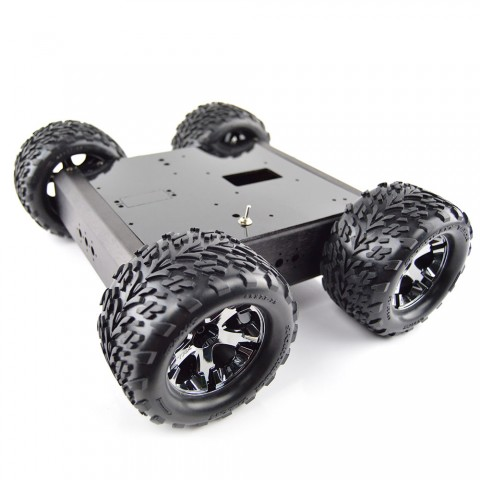
\includegraphics[width=0.25\textwidth]{lynxmotion-aluminum-a4wd1-rover-kit-w-encoders-7}
	\label{FigLynxmotionRover}
\end{wrapfigure}

The mobile base chosen was the Lynxmotion A4WD1 Rover, shown in Figure \ref{FigLynxmotionRover}. It was purchased as a kit including four 200 RPM DC gear motors, 100 PPR motor encoders, and 4.75" diameter wheels. The chassis consists of four aluminum side brackets, and two polycarbonate panels on the top and bottom. This kit makes up the bulk of the cost of the project. It was chosen for its larger wheels with relatively strong motors, making it robust to uneven terrain and ramps, ideal for outdoor use. The rover can support up to 5 lbs overall, and a second level which stacks on top is available as an extension. This second level would be an ideal place to put a tablet or small laptop.

One downside of this robot base is the fixed position of the four wheels. The lack of a turnable axis means the rover must steer by varying the speed of its motors. This causes wheel slippage in one or more of the wheels when the rover turns, meaning the motor encoders won't see the distance traveled. This ultimately causes errors in the robot's localization. Choosing a different base which uses only two driven wheels would avoid this issue, and likely be even cheaper. However, such a choice must be balanced with the robot's suitability for outdoor use, and room for all on-board components.

The motors are controlled by a Sabertooth dual-channel 12A 6V-24V regenerative motor driver. The lithium ion battery over-discharge protection.
protects from back EMF causing a current flow

There is a 5A version of this motor driver, which should have been purchased to save \$20.

This motor driver is powered by two LG 18650 HE2 rechargable lithium ion cells, which sit in an 18650 battery case. This case is made out of a battery holder soldered in series to act as a pack. The battery cells were individually charged before each use by a NiteCore-i2-V2014 li-ion charger.

\begin{wrapfigure}{r}{0.25\textwidth} %this figure will be at the right
	\caption{PING))) Ultrasonic Sensor \cite{fig_ping}}
	\centering
	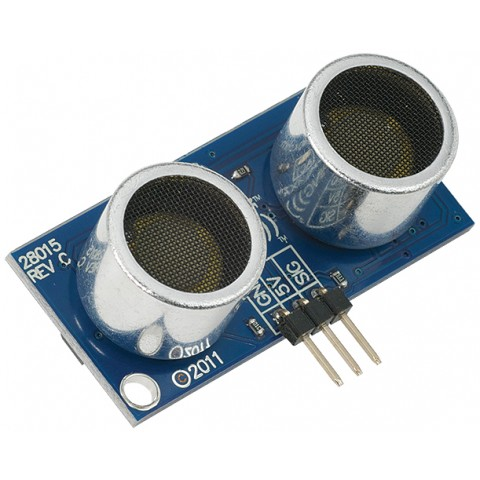
\includegraphics[width=0.25\textwidth]{parallax-ping-ultrasonic-sensor}
	\label{FigPing}
\end{wrapfigure}

On top of the rover is the PING))) ultrasonic distance sensor (see Figure \ref{FigPing}), which is attached to a standard Parallax servo which pans back and forth 180 degrees. This range sensor emits an ultrasonic chirp, and times how long it takes for that chirp to echo back. Based on that time, the distance from the sensor to an obstacle can be calculated. The PING))) sensor can be used to detect objects from 2cm to 3 meters away. \cite{pingDocumentation}

\begin{wrapfigure}{l}{0.25\textwidth}
	\caption{Arduino Uno R3 \cite{fig_arduino_uno}}
	\centering
	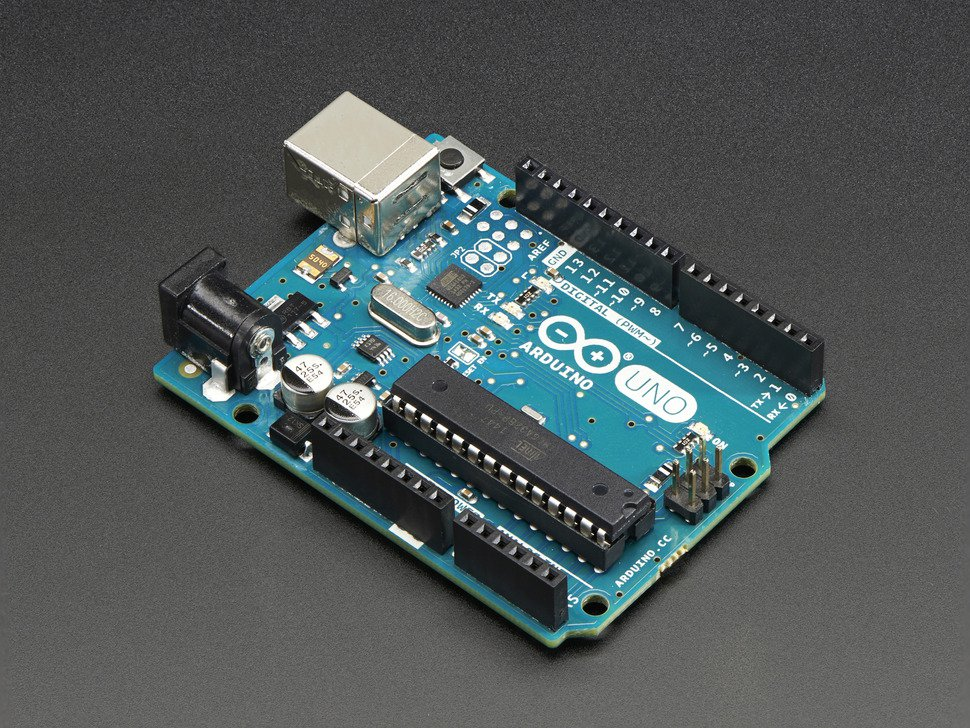
\includegraphics[width=0.25\textwidth]{arduinoUno}
	\label{FigArduino}
\end{wrapfigure}

At the center of the rover is an Arduino Uno R3, see Figure \ref{FigArduino}. This microcontroller board handles several important tasks. It tells the motor driver what speed to set its two output channels to, and directly controls the panning motion of the standard Parallax servo. It also acts as a go-between for the digital output of the sensors on the rover and a laptop. It's connected to this laptop via a USB cable, which powers the board and allows communication over a serial port. Motor encoder values and ultrasonic range data are transmitted to the laptop, and motor power commands are received. An Arduino prototyping shield is stacked on top to allow re-usability of the board.

Only two encoders end up being used, due to a limit of the microcontroller board used. Choosing a different model with more hardware interrupt pins would improve accuracy, without drastically increasing the price.

The specific laptop used in this project is the Dell Inspiron 3531, which has a quad core 2.16 GHz processor, and 4 GB of RAM. Any personal laptop running Ubuntu or Debian could be used here, and additional computational resources would be beneficial. However, this laptop was a personal work machine and already available to use at no additional cost. The laptop is used as the main processing unit for the navigation logic.

The last component is a Nexus 4 smartphone placed on the top panel of the rover, which is also connected to the laptop by USB. Inside this phone is an MPU-6050 chip which contains a gyroscope and accelerometer. Elsewhere on the phone's logic board are a magnetometer, otherwise known as a digital compass, and a GPS receiver. This was also a personal device already available, and acts as a cheap Inertial Measurement Unit (IMU) and GPS receiver for the robot.

\section{Construction}

\begin{wrapfigure}{r}{0.5\textwidth}
	\caption{Constructed Chassis}
	\centering
	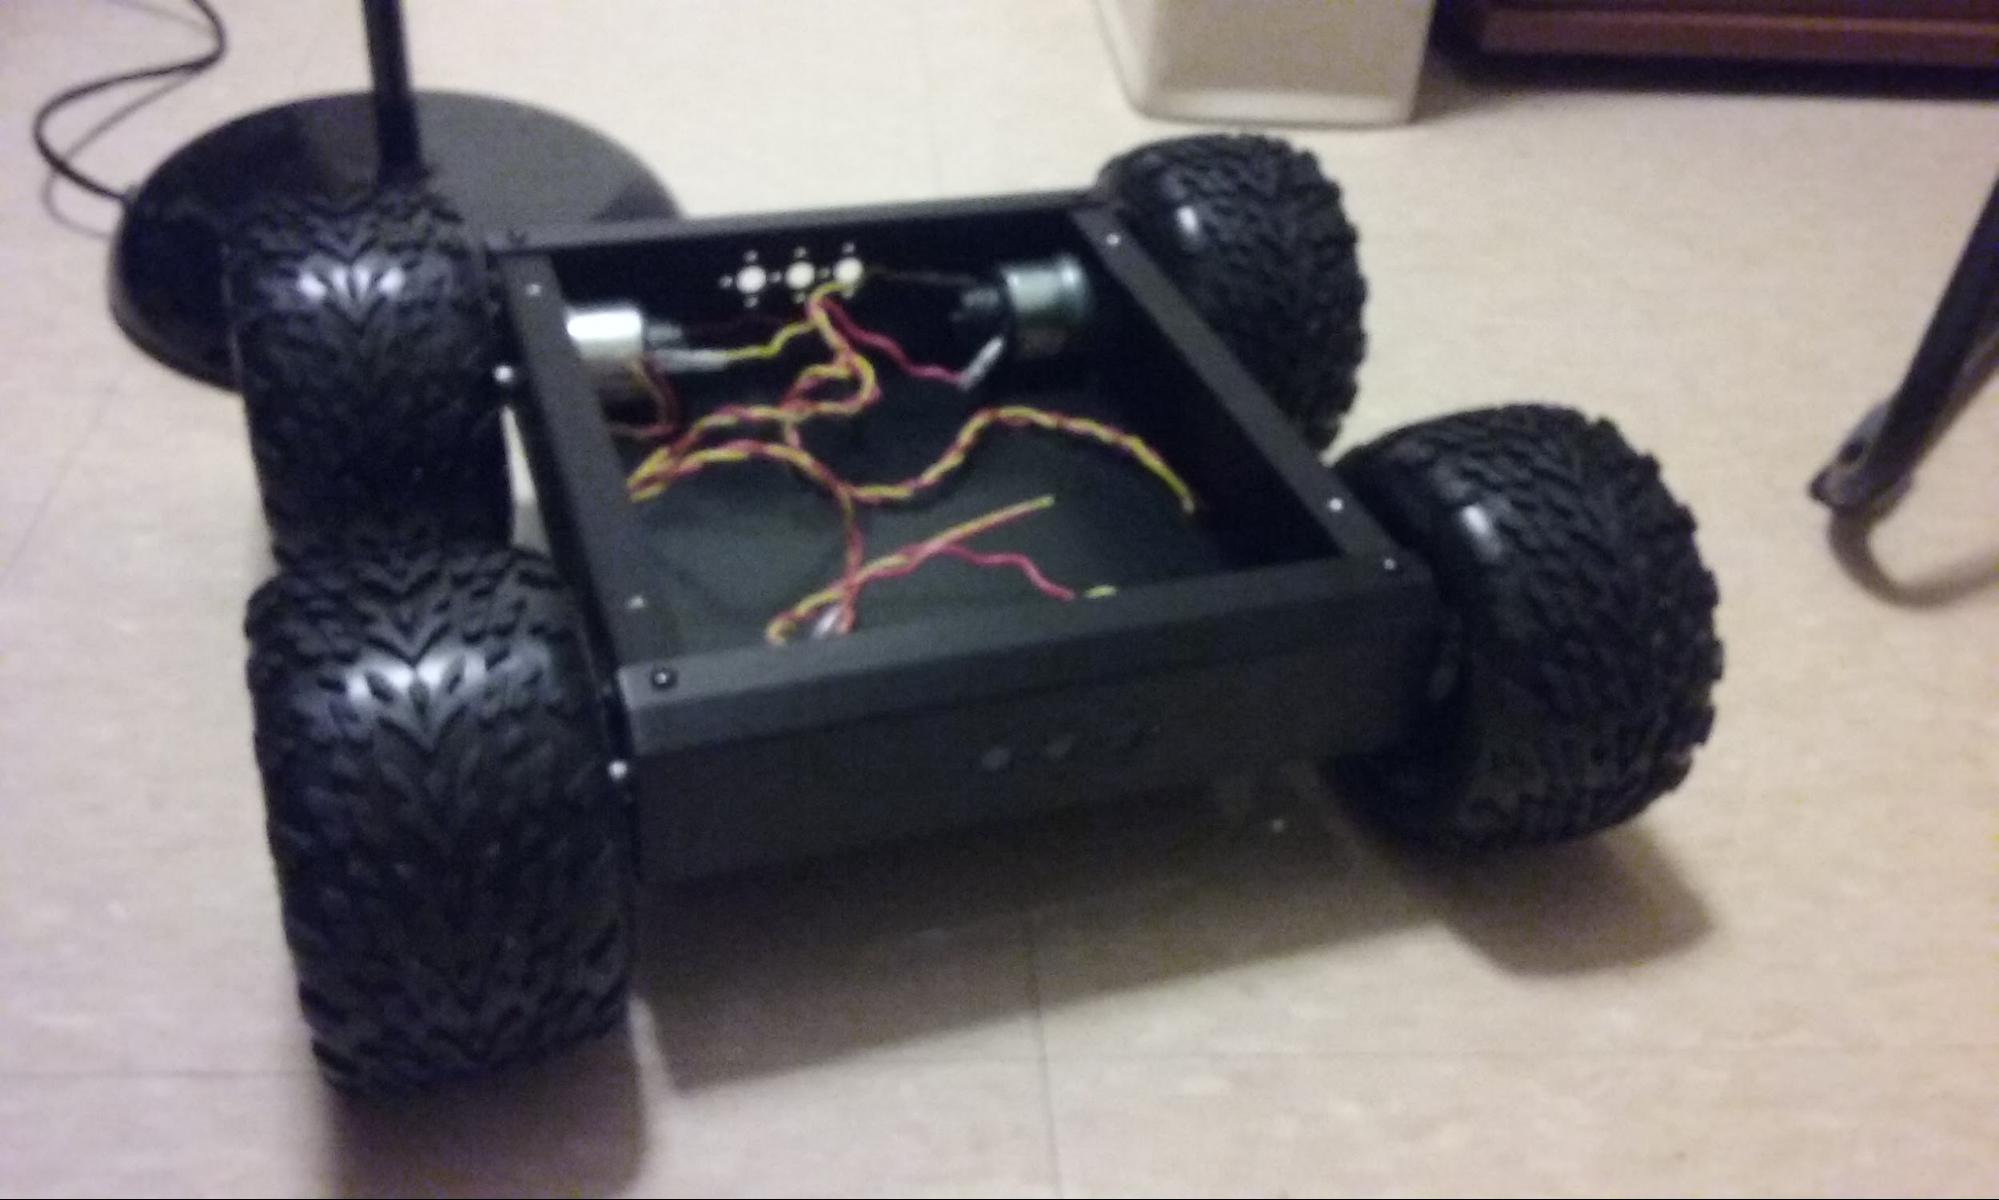
\includegraphics[width=0.5\textwidth]{chassis-constructed}
	\label{FigConstructedChassis}
\end{wrapfigure}

Figure \ref{FigConstructedChassis} shows the base just after assembly. The aluminum side brackets' mounting holes did not line up properly with the motors, so a Dremel drill was used to widen them.

\begin{wrapfigure}{l}{0.5\textwidth}
	\caption{Pieces Mounted}
	\centering
	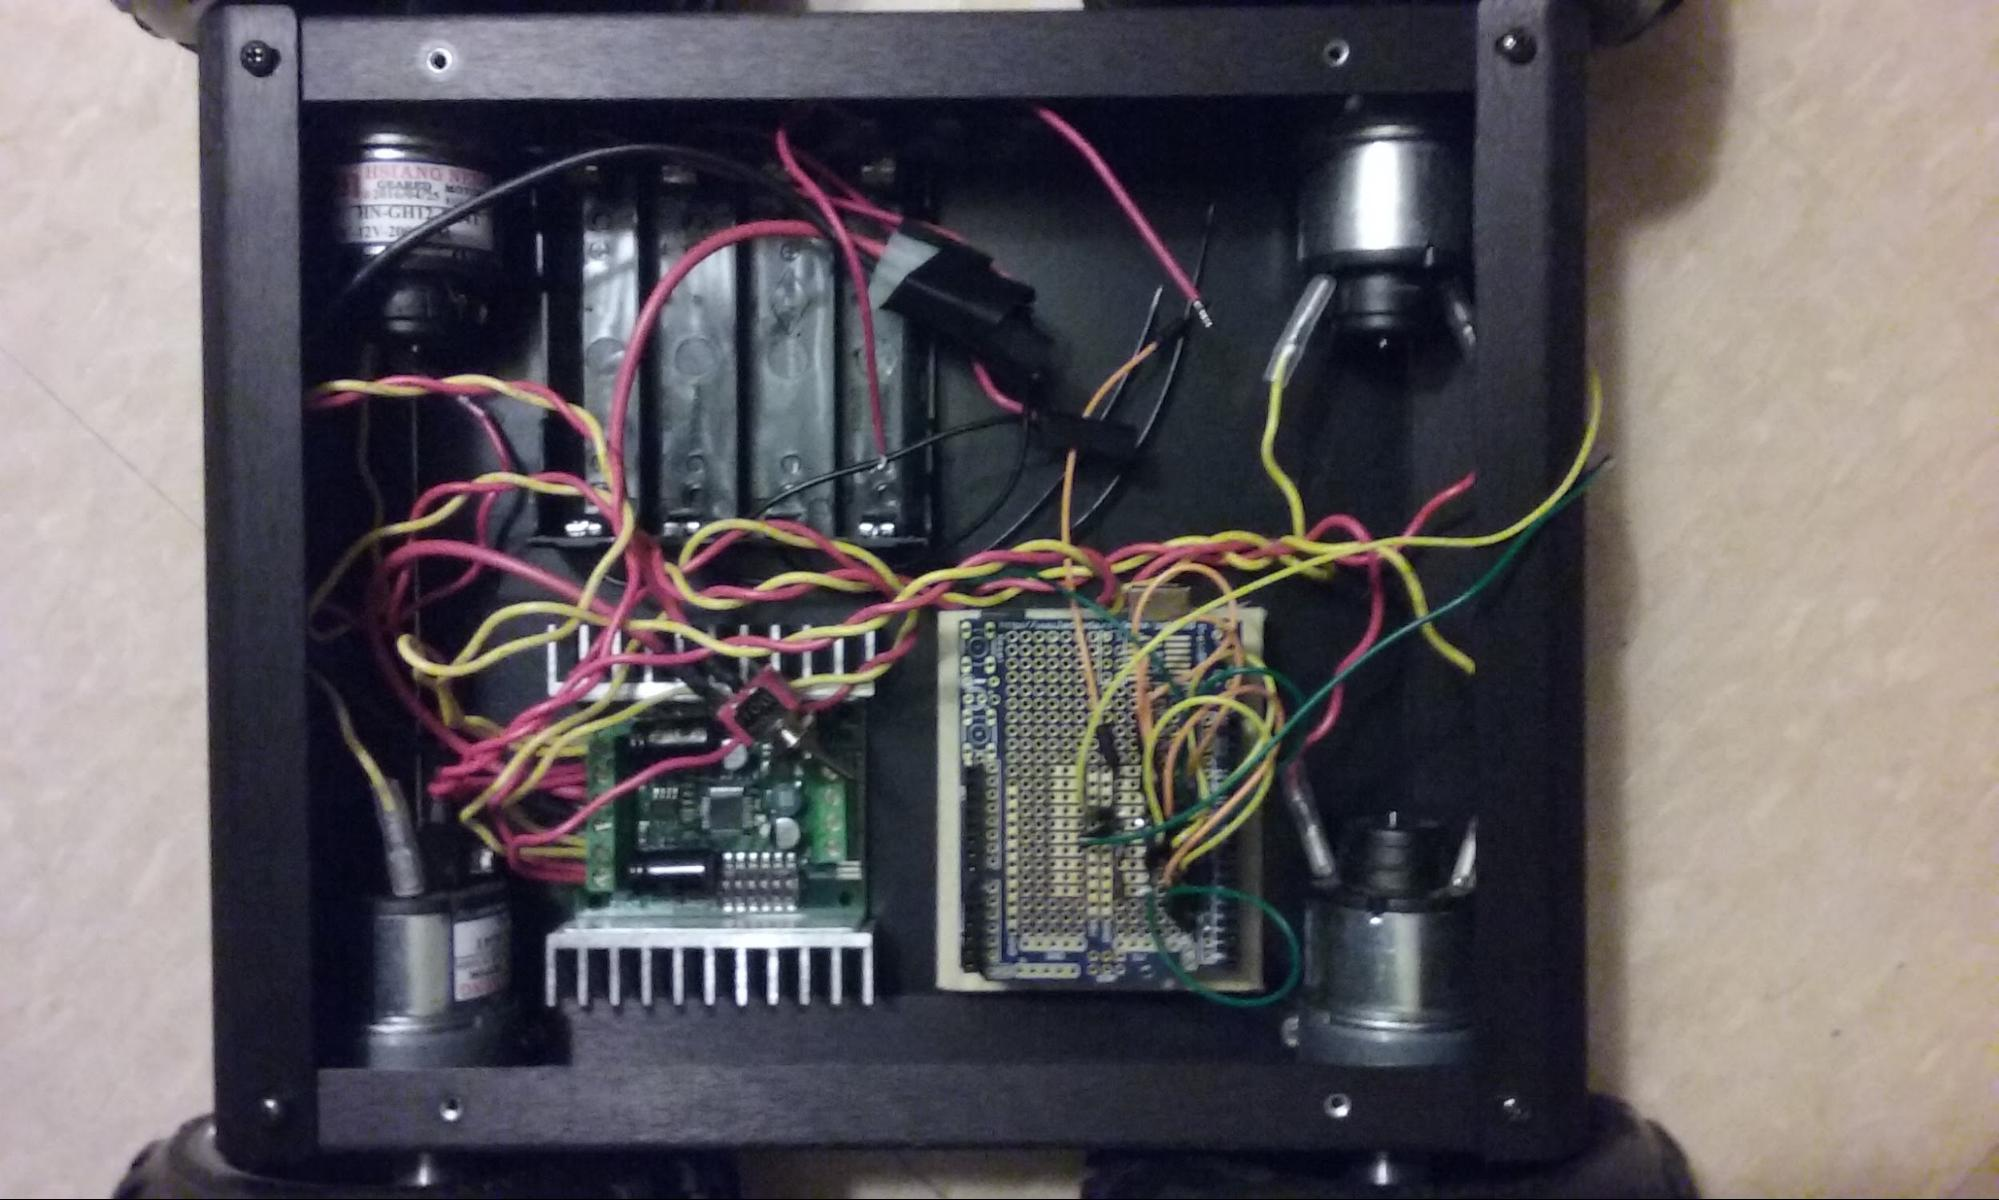
\includegraphics[width=0.5\textwidth]{chassis-parts-mounted}
	\label{FigChassisParts}
\end{wrapfigure}

The Arduino Uno was screwed to a 2.5" x 3" x 0.5" wooden poplar block, with non-conductive nylon washers placed between the screw head and the Uno, and between the Uno and the wooden block. The wooden Arduino mounting board and the Sabertooth were both attached via double-sided foam mounting tape to the bottom panel of the rover. The battery holder was attached with glue dots to make removal easier.

\begin{wrapfigure}{r}{0.5\textwidth}
	\caption{Construction Finished}
	\centering
	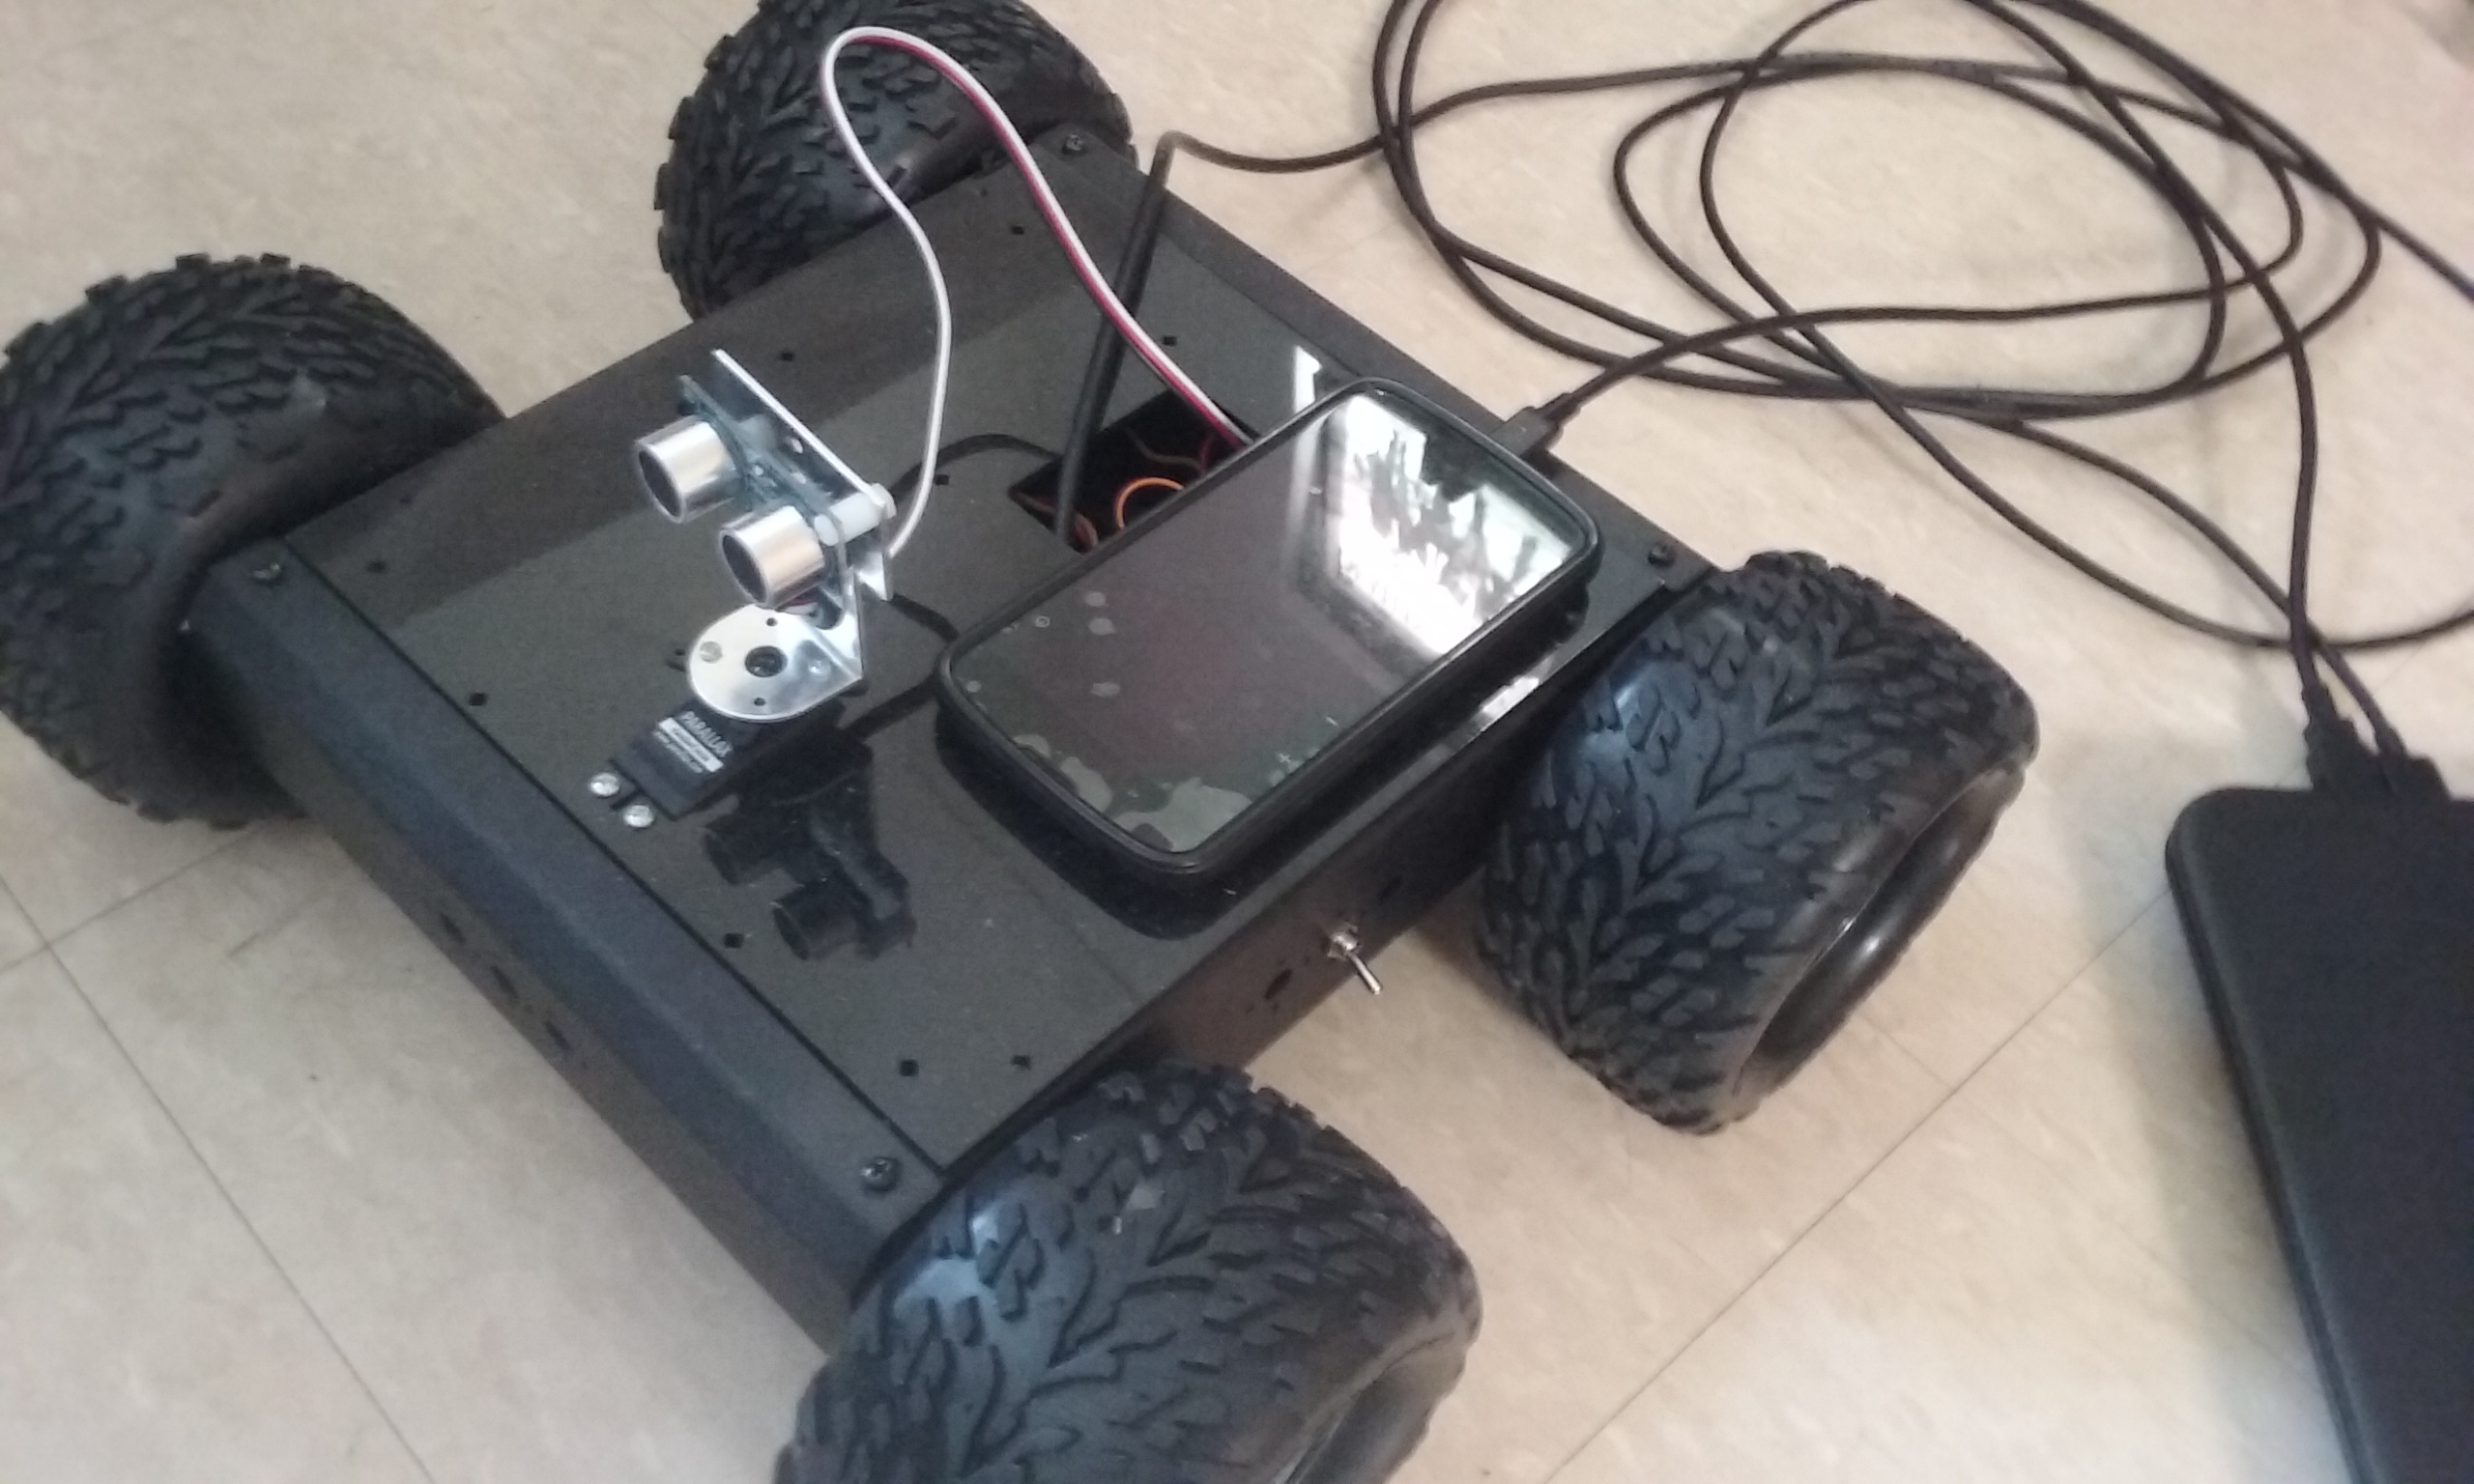
\includegraphics[width=0.5\textwidth]{roverFinished}
	\label{FigRoverFinished}
\end{wrapfigure}

The servo fits conveniently into a pre-cut opening in the top chassis panel, and is held in place with four 3mm x 6mm screws and corresponding washers. A mounting bracket is attached to the servo, and the PING))) sensor is screwed to that mounting bracket, using non-conductive washers and screws to separate the circuit board and the metal mounting bracket.

Another opening in the top panel allows the PING))) sensor to connect to the Arduino inside the body of the rover. This opening also allows the type A/B USB cable connected to the Arduino to extend out and reach the laptop. The smartphone sits on the top panel just to the left of this opening, secured in place by removable glue adhesive dots. It is also connected to the laptop via a micro-USB to USB cable.

Both USB cables are long, stretching to just under 10 feet. The USB 2.0 specification limits the length of cable between two 2.0 USB devices to less than five meters, or about 16 feet \cite{usbForum}. Thus there should be no problem with the current length, but extensions in the future could not go much further. 

Connecting electronics on the rover to the laptop via USB means the processing laptop must manually be kept within 10 feet of the rover as it navigates. This design could easily be extended to include wireless or radio communication with a server, and a larger chassis would simply be able to carry the laptop on it. However, USB cables are cheap and still function as a proof of concept for an autonomous design.

\begin{figure}[p] 
	\caption{Connections Made}
	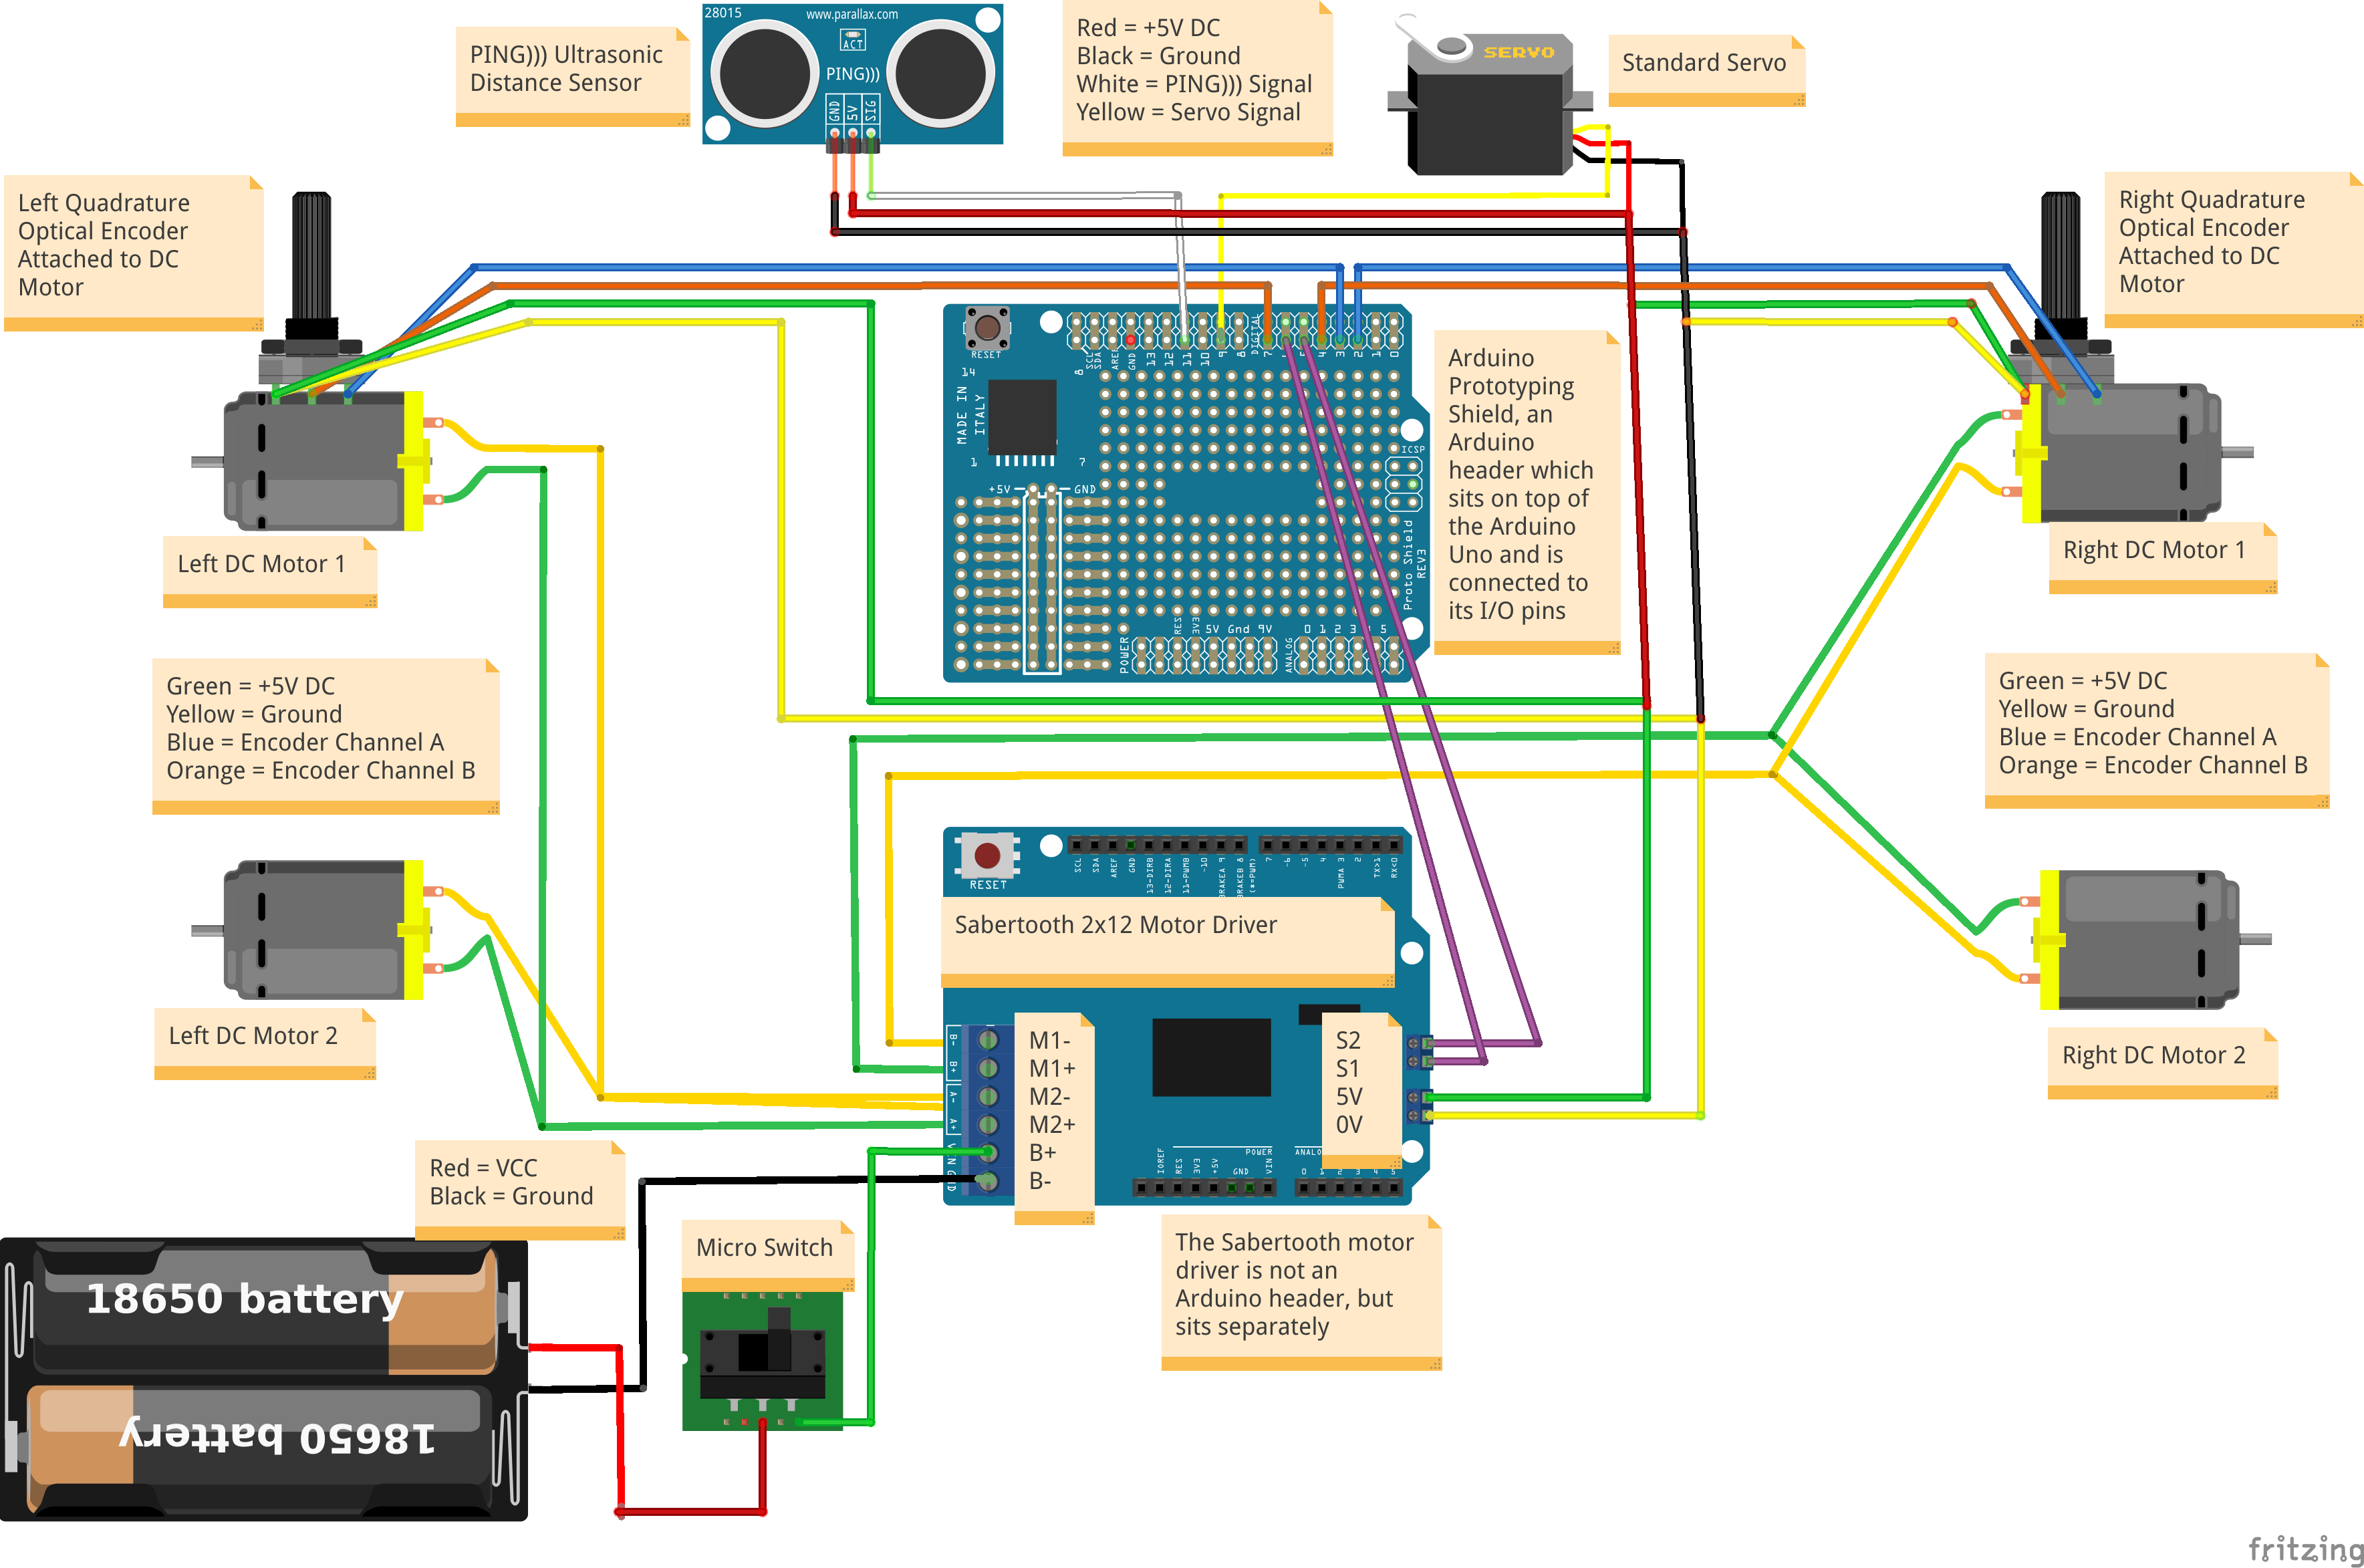
\includegraphics[width=\textwidth,height=\textheight,keepaspectratio, angle=0]{RoverDesign}
	\centering
	\label{figRoverDesign}
	\text{This image was created with Fritzing}
\end{figure}

Figure \ref{figRoverDesign} is a schematic specifying the overall design for the rover.

Connections were made with flexible stranded core, 22 AWG breadboard wires. Connections to the Arduino's digital pins were made indirectly. A prototyping shield was stacked on top of the Arduino, and connected to its digital pins via pin headers. Signal pins were then soldered to the prototyping shield. Breadboard wires needing direct connection ideally should use terminal block connectors. However, these were difficult to find at a reasonable price, and so wires were soldered together tip to tip, and then wrapped in electrical tape.

The Sabertooth motor driver controls two motor channels. It drives DC motors from these channels in a relatively simple way. The speed of DC motors is proportional to the voltage supplied to them, and the direction of rotation can be flipped simply by flipping the polarity of the supplied voltage. The motor driver manages the voltage supplied to each channel by using pulse-width modulation, which involves switching the power on and off at a high frequency. This approximates a smooth waveform of the average voltage and current. An on-board H-bridge is used to flip the polarity. \cite{dcMotorBlog}


\subsection{Power}
Besides the Arduino Uno, which is powered separately by a USB connection to the laptop, most of the rover's components are powered by the battery pack. This pack contains two individual 18650 lithium-ion cells placed into a battery holder and connected in series. The battery pack is then connected to the motor driver's battery terminals B+ and B-. The positive B+ output goes through a microswitch, which is attached to a side bracket in the rover, and is accessible from the outside. This acts as a kill switch for the battery pack.

Each 18650 cell holds 4.2V at full charge, and discharges down to a minimum of 2.7V. The motor driver has a lithium cutoff mode which shuts the driver down when the average voltage of cells in the battery pack reaches 3.0V. Thus the voltage supplied to the four motors through the motor driver's output channels will range from 8.4V to 6.0V, which is within their acceptable operating range.

The specific li-ion cells being used can supply up to 20A continuously, and the motor driver can handle up to 12A per channel. The motors each draw a maximum current of 1.5A, and two are used per channel, putting the total possible current draw of 3A per channel well below the limits of the motor driver and battery pack.

The motor driver has an onboard battery eliminator circuit (BEC) which is an efficient 5V voltage regulator capable of supplying up to 1 amp of continuous current, with 1.5 Amps at peak. The ultrasonic sensor, its servo, and the two rotary encoders combined use less than 500 mA, and are all powered through this BEC.  The Arduino is also connected to this BEC's ground, as the Uno and Sabertooth must share a common ground plane in order for the control signals to be interpreted correctly \cite{sabertoothUserGuide}. It's important to note that a BEC of some kind is essential in this project, as the Arduino's on-board 5V regulator can not handle the peak amperage draw of the servo, and if used risks overheating.

The standard servo has the potential to draw peak currents of up to 1A, if it hits a snag and is stopped from moving. Therefore the input wires to the 5V and 0V BEC terminal connectors should be capable of handling those peaks. Since we are using 22 AWG wires, we are close to the limit, but a 22 AWG wire with 43 or more internal cores is rated to handle 1A. And the expected consistent draw is much lower, less than 500mA. 

Note that the sensors attached to the microcontroller should be powered off before the Arduino, else the Arduino may try to power the whole Mega chip via its input pins. The sensors are powered from the BEC on the motor driver, so they may be turned off by using the microswitch between the battery holder and the motor driver.

